\documentclass[letterpaper,10pt]{article}
\usepackage[utf8]{inputenc}
\usepackage{amsmath}
\usepackage{amssymb}
\usepackage{graphicx}
\usepackage{listings}
\usepackage{float}
\usepackage{natbib}
\bibliographystyle{plainnat}

\newcommand{\dd}{\,\mathrm{d}\,}
\newcommand{\pp}{\partial}
\newcommand{\co}{\mathrm{.}}
\newcommand{\cosec}{\mathrm{cosec}}
\newcommand{\cotan}{\mathrm{cotan}}
\newcommand{\D}{\displaystyle}

\renewcommand{\vec}[1]{\boldsymbol#1}
\newcommand{\bhat}[1]{\hat{\boldsymbol#1}}

\setlength\headheight{0in}
\setlength\headsep{0in}
\setlength\textheight{9in}
\setlength\textwidth{6.5in}
\setlength\oddsidemargin{0in}
\setlength\evensidemargin{0in}
\setlength\parindent{0.25in}
\setlength\parskip{0.25in}

%opening
\title{Test Cases}
\author{Pablo Marchant Campos}
\begin{document}
\maketitle

In my notation, the axisymmetric field is written as
\begin{eqnarray}
\vec{B}=\beta\nabla\phi+\nabla\alpha\times\nabla\phi,
\end{eqnarray}
while on Jaime's notation, the expression used is
\begin{eqnarray}
\vec{B}=B_t\bhat{\phi}+\nabla\times(A\bhat{\phi}).
\end{eqnarray}
Both choices are related by
\begin{eqnarray}
B_t=\frac{\beta}{r\sin\theta},\quad A=\frac{\alpha}{r\sin\theta}.
\end{eqnarray}
The following will follow the $\alpha,\beta$ notation.

We are interested in time-evolving the equation
\begin{eqnarray}
\frac{\dd \vec{B}}{\dd t}=-\nabla\times\left([\nabla\times\vec{B}]\times\vec{B}\right)-R_B^{-1}\nabla\times\left(\nabla\times\vec{B}\right),
\end{eqnarray}
where the dimensionless magnetic field $\vec{B}$ is chosen to have a characteristic value of $1$ (the specific way in which this is done will be specified later).

We are interested in using Ohm modes as initial conditions. For this particular case of constant resistivity, both the time evolution equation for $\alpha$ and $\beta$ are the same,
\begin{eqnarray}
\frac{\pp \alpha}{\pp t}=R_B^{-1}\Delta\alpha,\quad \frac{\pp \beta}{\pp t}=R_B^{-1}\Delta\alpha,
\end{eqnarray}
For which the separable (axisymmetric) solutions are
\begin{eqnarray}
\alpha=\left(Aj_l\left(\frac{r}{\sqrt{\tau R_B^{-1}}}\right)+By_l\left(\frac{r}{\sqrt{\tau R_B^{-1}}}\right)\right)P_l^1(\cos\theta)r\sin\theta e^{-t/\tau},\\
\beta=\left(Cj_l\left(\frac{r}{\sqrt{\tau R_B^{-1}}}\right)+Dy_l\left(\frac{r}{\sqrt{\tau R_B^{-1}}}\right)\right)P_l^1(\cos\theta)r\sin\theta e^{-t/\tau}.
\end{eqnarray}
We are interested in modes restricted to a shell with adimensional internal radius $r_{min}=0.75$. For the boundary conditions, we take two possible options, explained in each of the following sections.

\section*{Zero-Boundary conditions}
This is the simplest case, where I require
\begin{eqnarray}
\beta(r_{min},\theta)=\beta(1,\theta)=\alpha(r_{min},\theta)=\alpha(1,\theta)=0.
\end{eqnarray}
For this case, since the functional form of $\alpha$ and $\beta$ are the same, the timescale $\tau$ will be the same for both. If we take the boundary condition on $\beta$, we have
\begin{eqnarray}
Cj_l(kr_{min})+Dy_l(kr_{min})=0\\
Cj_l(k)+Dy_l(k)=0,
\end{eqnarray}
where $k\equiv(\tau R_B^{-1})^{-1/2}$. This two conditions can be transformed into a trascendental equation for $k$, and an equation that gives $B$ in terms of $C$ and $k$,
\begin{eqnarray}
j_l(kr_{min})y_l(k)-y_l(kr_{min})j_l(k)=0\\
C=-\frac{Dy_l(k)}{j_l(k)},
\end{eqnarray}
and for $\alpha$, we obtain the same equation for $k$, and a similar one that gives $A$ in terms of $B$ and $k$,
\begin{eqnarray}
A=-\frac{By_l(k)}{j_l(k)}.
\end{eqnarray}
Using this, together with requiring that $|\vec{B}|\sim 1$ at the point where the field is stronger, we obtain the following values for the first modes with $r_{min}=0.75$ ($n$ represents the radial mode, being $n=1$ the fundamental mode):
\begin{table}[h!]
\begin{center}
\begin{tabular}{cc|ccccc}
n&l&k&A&B&C&D\\
\hline
1&1& 12.67071 & -0.13731 & 0.74154 & -2.00235 & 10.81346 \\
2&1& 25.18557 & -0.06938 & 0.74784 & -1.88596 & 20.32767\\
1&2& 12.87682 &  0.43501 & 0.26278 &  6.32868 &  3.82300\\
2&2& 25.29089 &  0.48296 & 0.13719 & 13.11642 &  3.72583
\end{tabular}
\end{center}
\end{table}
The poloidal modes in these case are somewhat singular, because they do not have $B_\theta=0$ at the surface and the inner radius (being the latter the place where the maximum intensity of the field is reached).
\section*{Non-zero boundary conditions}
In order to consider cases where magnetic flux is allowed to exit the star, we must have that the field is completely continuous along the surface of the star. In order for this to be satisfied, it is enough that the $r$ and $\theta$ derivatives of $\alpha$ be continuous. Outside the star, since there are no currents, we must have
\begin{eqnarray}
\nabla\cdot(\nabla\alpha\times\nabla\phi)=0,
\end{eqnarray}
which, for axisymmetric configurations gives the separable solutions
\begin{eqnarray}
\alpha=\frac{E}{r^l}P_l^{1}(\cos\theta)\sin\theta.
\end{eqnarray}
Applying the required boundary conditions then means applying simultaneously the following three conditions:
\begin{itemize}
\item Continuity of the $\theta$ derivative, this only requires $\alpha$ to be continuous, i.e.
\begin{eqnarray}
Aj_l(k)+By_l(k)=E
\end{eqnarray}
\item Continuity of the $r$ derivative,
\begin{eqnarray}
Aj_l(k)+By_l(k)+k(Aj_l'(k)+By_l'(k))=-El,
\end{eqnarray}
which can be simplified by using the first boundary condition,
\begin{eqnarray}
Aj_l'(k)+By_l'(k)=-\frac{C}{k}(l+1),
\end{eqnarray}
\item Zero boundary condition at the inner radius,
\begin{eqnarray}
Aj_l(kr_{min})+By_l(kr_{min})=0.
\end{eqnarray}
\end{itemize}
As was the case with the zero boundary conditions on the surface, this set of boundary conditions can be modified to be a trascendental equation for $k$, and two equations which give the values of $A$ and $B$ in terms of the value of $C$,
\begin{eqnarray}
\begin{aligned}
\left(\frac{y_l(k)}{k}(l+1)+y_l'(k)\right)j_l(kr_{min})-\left(\frac{j_l(k)}{k}(l+1)+j_l'(k)\right)y_l(kr_{min})=0\\
A=\frac{\frac{E}{k}(l+1)y_l(k)+Ey_l'(k)}{y_l'(k)j_l(k)-y_l(k)j_l'(k)},\qquad
B=\frac{-\frac{E}{k}(l+1)j_l(k)-Ej_l'(k)}{y_l'(k)j_l(k)-y_l(k)j_l'(k)},
\end{aligned}
\end{eqnarray}
however, since the value of $E$ holds no value to us, we can redefine it to include the common factors involved, so we have simplified expressions for $A$ and $B$,
\begin{eqnarray}
\begin{aligned}
A=E\left(\frac{(l+1)}{k}y_l(k)+Ey_l'(k)\right),\qquad
B=-E\left(\frac{(l+1)}{k}j_l(k)+j_l'(k)\right).
\end{aligned}
\end{eqnarray}
Using this expressions, and once again requiring that $|\vec{B}|\sim 1$ at the point where the field is stronger, I get the following values for the first modes:
\begin{table}[h!]
\begin{center}
\begin{tabular}{cc|ccc}
n&l&k&A&B\\
\hline
1&1&  7.03266 & -0.55882 & -0.52004\\
2&1& 19.12793 & -0.72288 & -0.20659\\
1&2&  7.81795 & -0.52101 & -0.04764\\
2&2& 19.46616 & -0.31188 &  0.39534
\end{tabular}
\end{center}
\end{table}

\section*{List of cases to test}
\subsection*{Pure Ohm evolution}
For pure Ohm evolution, we will consider all modes listed before, with $R_B=1,10,100$, to verify that the solved timescales scale correctly with $R_B$.
\subsection*{Hall+Ohm}
All of the following cases shoudl be evolved considering $R_B=25,50,100,200$.
\subsubsection*{Purely toroidal or poloidal initial configurations}
In the case of either purely toroidal or purely poloidal initial configurations, we will evolve each of the modes listed before, for the specified values of $R_B$.
\subsubsection*{Mixed toroidal and poloidal initial conditions}
In the case of mixed initial conditions, lets consider $\alpha_{n,l,in}$, $\alpha_{n,l,out}$ and $\beta_{n,l}$ to be the modes listed before, where $in$ and $out$ denote the modes with magnetic field contained inside the star, and with field outside the star respectively. We will consider the following combinations for the total magnetic field
\begin{itemize}
\item Both fields with similar strengths,
\begin{eqnarray}
\vec{B}=\beta_{n,l}\times\nabla\phi+\nabla\alpha_{n,l,in}\times\nabla\phi,\quad\vec{B}=\beta_{n,l}\times\nabla\phi+\nabla\alpha_{n,l,out}\times\nabla\phi,\quad
\end{eqnarray}
\item Cases with a stronger poloidal field,
\begin{eqnarray}
\vec{B}=0.6\beta_{n,l}\times\nabla\phi+\nabla\alpha_{n,l,in}\times\nabla\phi,\quad\vec{B}=0.6\beta_{n,l}\times\nabla\phi+\nabla\alpha_{n,l,out}\times\nabla\phi,\quad\\
\vec{B}=0.3\beta_{n,l}\times\nabla\phi+\nabla\alpha_{n,l,in}\times\nabla\phi,\quad\vec{B}=0.3\beta_{n,l}\times\nabla\phi+\nabla\alpha_{n,l,out}\times\nabla\phi,\quad
\end{eqnarray}
\item Cases with a stronger toroidal field,
\begin{eqnarray}
\vec{B}=\beta_{n,l}\times\nabla\phi+0.6\nabla\alpha_{n,l,in}\times\nabla\phi,\quad\vec{B}=\beta_{n,l}\times\nabla\phi+0.6\nabla\alpha_{n,l,out}\times\nabla\phi,\quad\\
\vec{B}=\beta_{n,l}\times\nabla\phi+0.3\nabla\alpha_{n,l,in}\times\nabla\phi,\quad\vec{B}=\beta_{n,l}\times\nabla\phi+0.3\nabla\alpha_{n,l,out}\times\nabla\phi,\quad.
\end{eqnarray}
\end{itemize}
In total, these means running $160$ different cases if we take into account all modes mentioned. Probably, for the sake sanity, we should just consider the fundamental modes for now $n=l=1$, and only $R_B=50,100,200$, which would reduce this to only $30$ simulations.

\pagebreak

\begin{figure}
\begin{center}
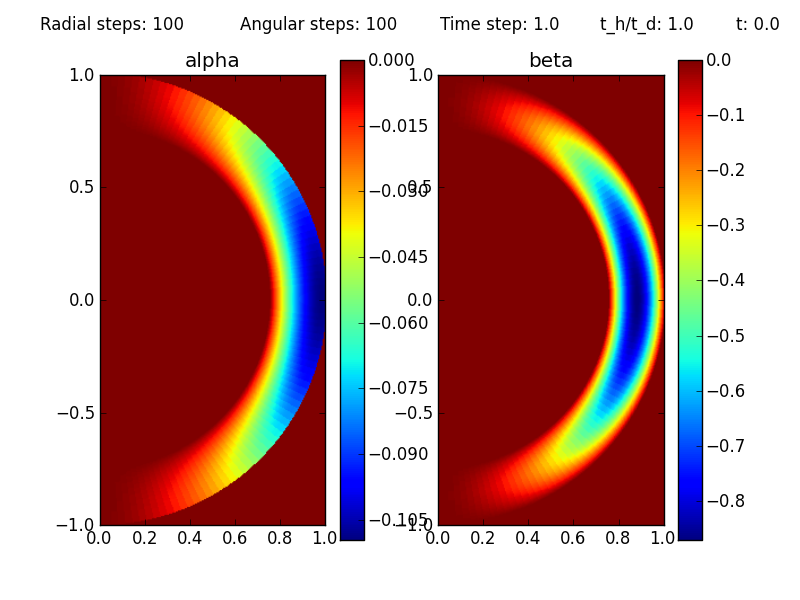
\includegraphics[scale=0.6]{tests/plot_0}
\caption{Modes with $l=1,n=1$. For the poloidal mode, we consider the one that has magnetic field outside the star.}
\end{center}
\end{figure}

\begin{figure}
\begin{center}
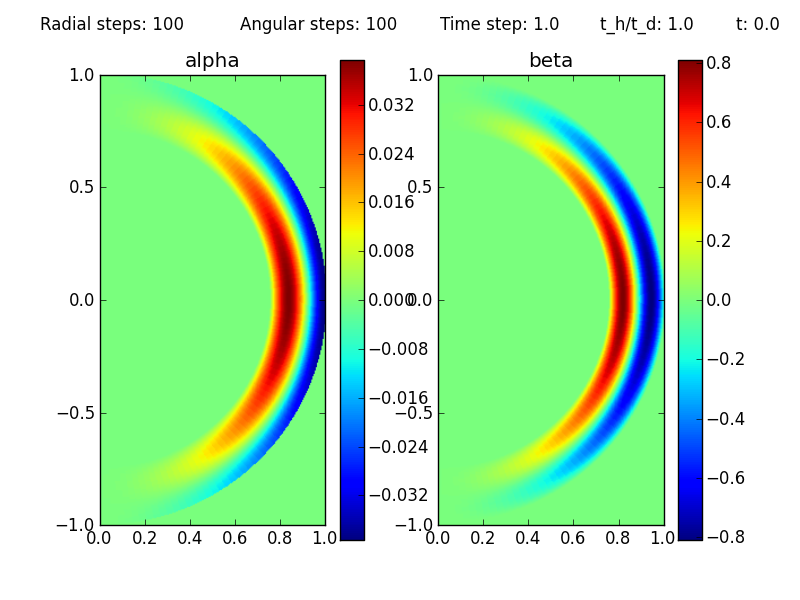
\includegraphics[scale=0.6]{tests/plot_1}
\caption{Modes with $l=1,n=2$. For the poloidal mode, we consider the one that has magnetic field outside the star.}
\end{center}
\end{figure}

\begin{figure}
\begin{center}
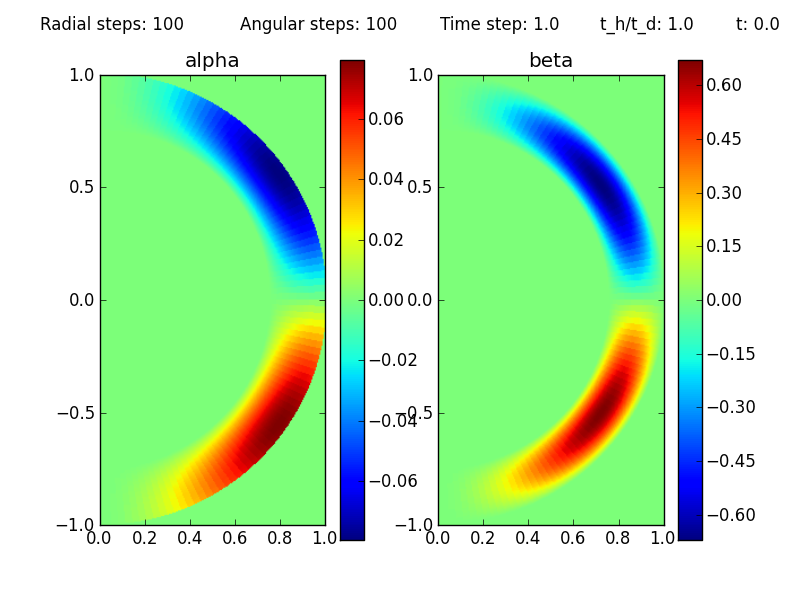
\includegraphics[scale=0.6]{tests/plot_2}
\caption{Modes with $l=2,n=1$. For the poloidal mode, we consider the one that has magnetic field outside the star.}
\end{center}
\end{figure}

\begin{figure}
\begin{center}
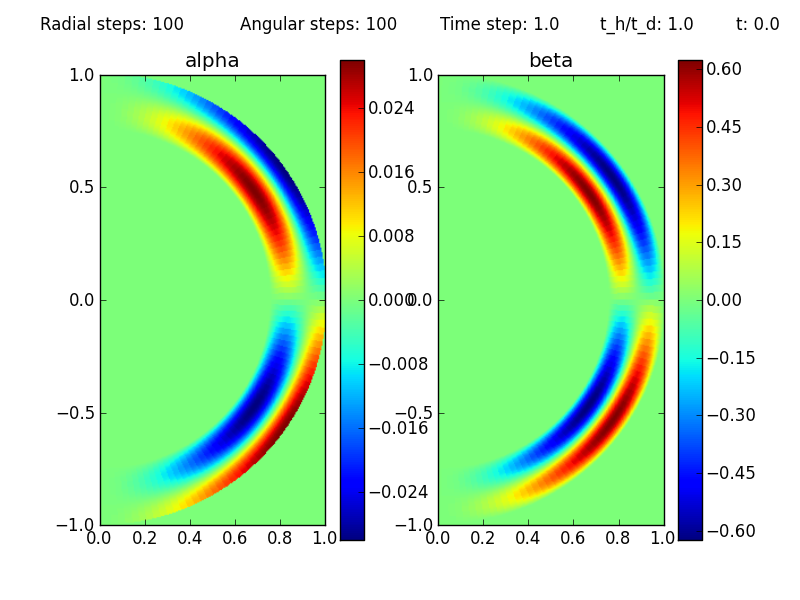
\includegraphics[scale=0.6]{tests/plot_3}
\caption{Modes with $l=2,n=2$. For the poloidal mode, we consider the one that has magnetic field outside the star.}
\end{center}
\end{figure}
\end{document}